\subsection{Behavior}
\label{sec:setup.arch.behavior}

\Cref{fig:setup.arch.period} shows the 2D scans of the periods \hl{associated wit parameter regions in the archetypal model}.
As before, \Cref{fig:setup.arch.period.halved} shows the \hl{halved} model to indicate ``type B'' parameter regions.
The structure \hl{is not very different from the previous constructed model in} \Cref{sec:setup.quad.hyper.2}.
There are still chains of parameter regions \hl{associated} with the same period next to each other \hl{with the period increasing by two for each chain}.
\hl{And the types of the parameter regions in each chain alternate between ``type A'' and ``type B''}.
Now the ``type B'' parameter regions are even more prominent in the chains for larger values of $\beta$.
This was not the case in the \hl{previous model with four quadratic branches}.

\Cref{fig:setup.arch.cobwebs} \hl{shows cobweb diagrams at the parameter values that are marked with points in} \Cref{fig:setup.arch.period}, \hl{as also done in previous sections of this chapter}.
\hl{
	Here, the model also behaves like the original model with the symbolic sequence of the cycle at the point $A$ being $\A^6\B^3\C^6\D^3$, at the point $C$ being $\A^5\B^4\C^5\D^4$, and in between both parameter regions associated with each cycle, two coexisting cycles with the symbolic sequences $\A^6\B^3\C^5\D^4$ and $\A^5\B^4\C^6\D^3$ at the point $C$.
	The next chapter covers the behavior of the archetypal model in-depth.
}

\begin{figure}
	\centering
	\subfloat[Model]{
		\includegraphics[width=.45 \textwidth]{50_Quadratic_linearR/2D_Period_Whole/result.png}
		\label{fig:setup.arch.period.full}
	}
	\subfloat[Halved Model]{
		\includegraphics[width=.45 \textwidth]{51_Quadratic_linearR_Halved/2D_Period_Whole/result.png}
		\label{fig:setup.arch.period.halved}
	}
	\caption[2D scans of the periods of the archetypal model]{
		2D scan of the periods of the \hl{archetypal model} with \hl{compound parameters} $g_R\left(\frac{1}{4}\right)$ and $g_R\left(\frac{1}{2}\right)$.
		The parameters $a_L = 4, b_L = -\frac{1}{2},$ and $g_R\left(\frac{1}{4}\right) = 0.525$ are fixed.
		The parameters $\alpha = -g_R\left(\frac{1}{4}\right)$ and $\beta = c_L$ are varied in the ranges $[-0.45, -0.275]$ and $[0.15, 0.1875]$, respectively.
		The points $A, B,$ and $C$ mark the parameter values used for the cobweb diagrams in \Cref{fig:setup.arch.cobwebs}.
		(a) shows the scan for the model as defined above, while (b) shows the scan for the halved model where we can see ``type B'' parameter regions as they have higher periods than the ``type A'' parameter regions of the same chain.
	}
	\label{fig:setup.arch.period}
\end{figure}

\begin{figure}
	\centering
	\begin{subfigure}{0.3\textwidth}
		\centering
		\includegraphics[width=\textwidth]{50_Quadratic_linearR/Cobweb_A/result.png}
		\caption{At point $A$}
		\label{fig:setup.arch.cobweb.A}
	\end{subfigure}
	\begin{subfigure}{0.3\textwidth}
		\centering
		\includegraphics[width=\textwidth]{50_Quadratic_linearR/Cobweb_B/result.png}
		\caption{At point $B$}
		\label{fig:setup.arch.cobweb.B}
	\end{subfigure}
	\begin{subfigure}{0.3\textwidth}
		\centering
		\includegraphics[width=\textwidth]{50_Quadratic_linearR/Cobweb_C/result.png}
		\caption{At point $C$}
		\label{fig:setup.arch.cobweb.C}
	\end{subfigure}
	\caption[Cobwebs of the piecewise hybrid quadratic model with hyperparameters]{
		Cobweb diagrams at three parameter values of $\alpha = -g_R\left(\frac{1}{4}\right)$ and $\beta = c_L$ in the piecewise hybrid quadratic model with hyperparameters.
		The other parameters are fixed as $a_L = 4, b_L = -\frac{1}{2},$ and $g_R\left(\frac{1}{2}\right) = \frac{1}{2} + \frac{1}{40}$.
		The parameter values are marked in \Cref{fig:setup.arch.period}.
	}
	\label{fig:setup.arch.cobwebs}
\end{figure}
